\documentclass[border=10pt]{standalone}
\usepackage[svgnames]{xcolor}
\usepackage{amsmath}
\usepackage{pgfplots}
\pgfplotsset{compat=newest}
\usepackage[sfdefault]{FiraSans}
\usepackage{FiraMono}
\renewcommand*\familydefault{\sfdefault}
\begin{document}
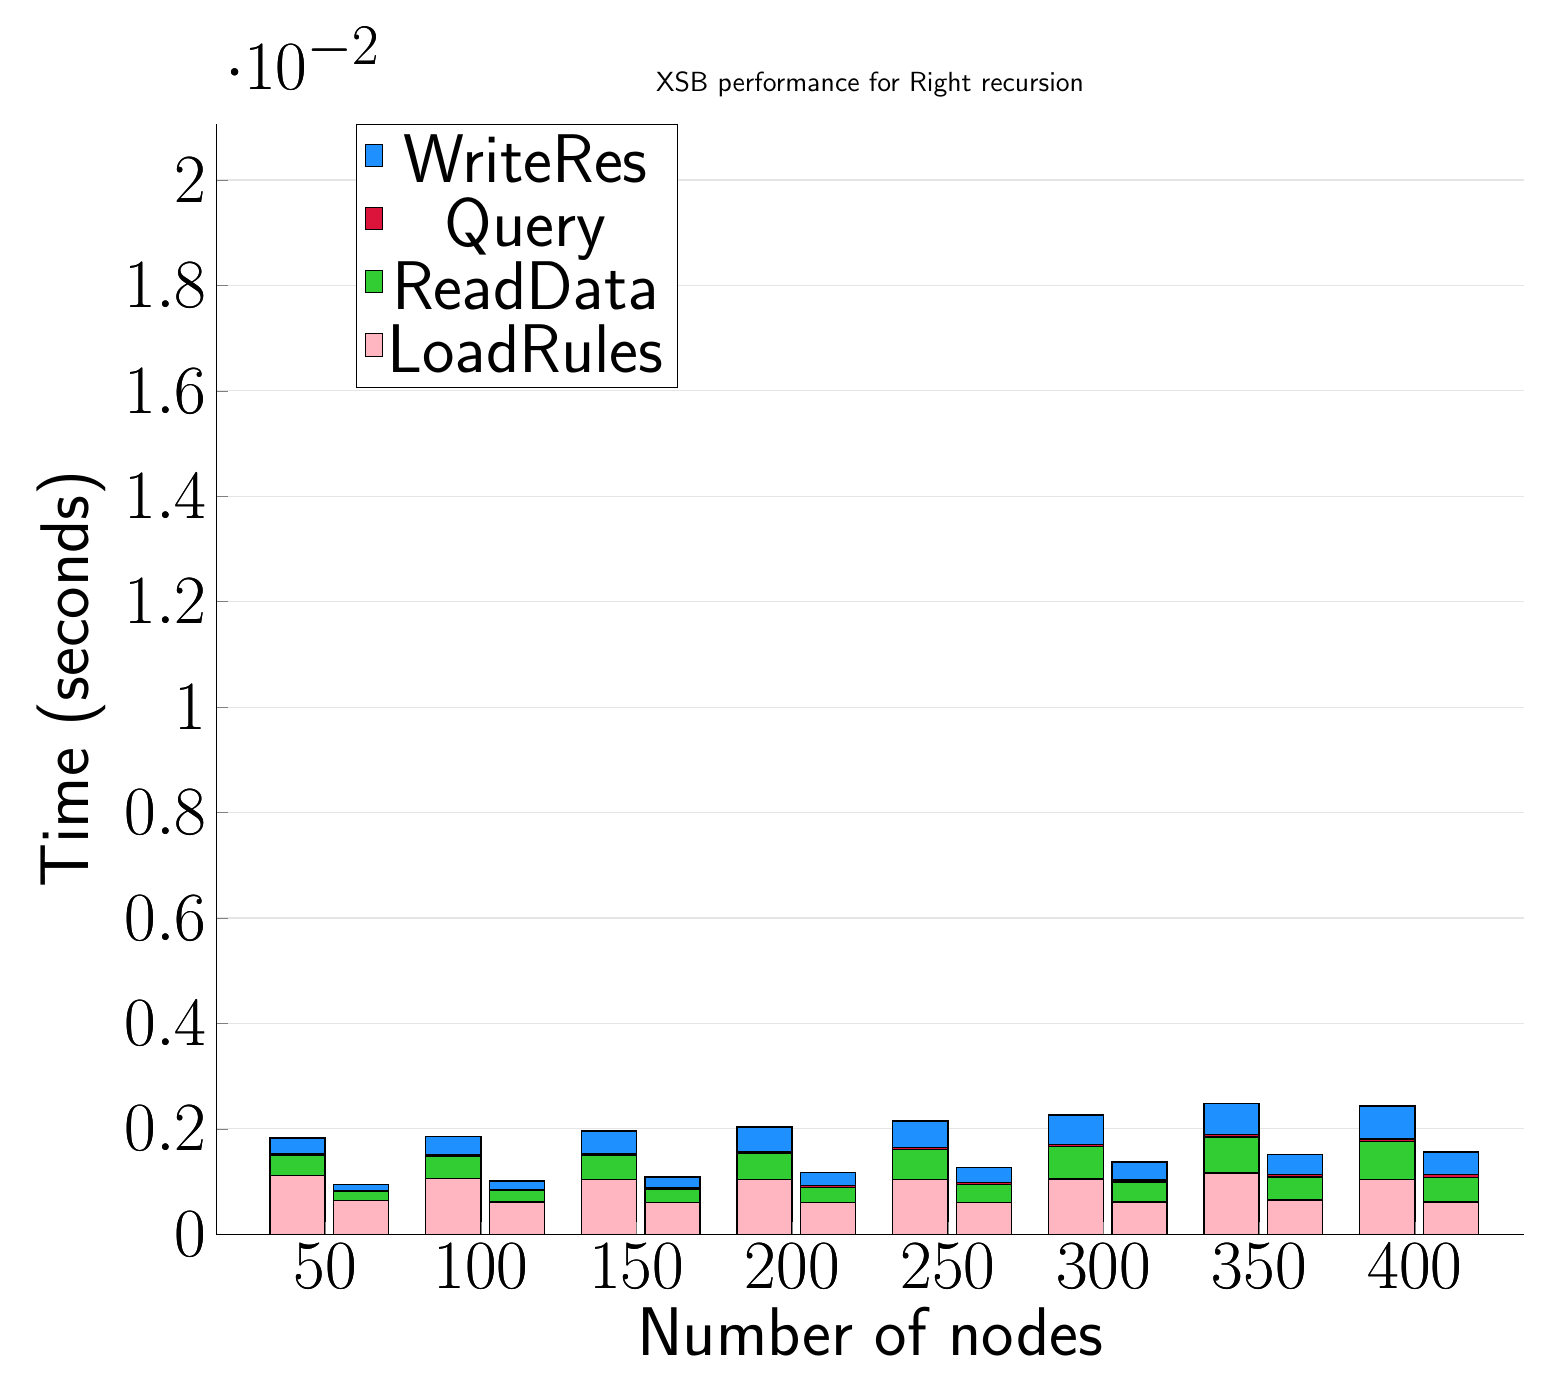
\begin{tikzpicture}
	\begin{axis}[
			ybar stacked,
			title={XSB performance for Right recursion},
			bar shift=-10pt,
			width=1.5\textwidth,
			bar width=0.7cm,
			ymajorgrids, tick align=inside,
			major grid style={draw=gray!20},
			xtick=data,
			ymin=0, ymax=0.021072192192077635,
			axis x line*=bottom,
			axis y line*=left,
			enlarge x limits=0.1,
			legend style={
					at={(0.23, 1)},
					anchor=north,
					legend columns=1,
					font=\Huge,
				},
			ylabel={Time (seconds)},
			xlabel={Number of nodes},
			label style={font=\Huge},
			tick label style={font=\Huge},
		]
		\addlegendimage{fill=DodgerBlue, draw=black, line width=0.2pt}
		\addlegendentry{WriteRes}
		\addlegendimage{fill=Crimson, draw=black, line width=0.2pt}
		\addlegendentry{Query}
		\addlegendimage{fill=LimeGreen, draw=black, line width=0.2pt}
		\addlegendentry{ReadData}
		\addlegendimage{fill=LightPink, draw=black, line width=0.2pt}
		\addlegendentry{LoadRules}
		\addplot +[fill=LightPink, draw=black, line width=0.5pt] coordinates {
				(50, 0.0011086225509643562)
				(100, 0.001054048538208008)
				(150, 0.001032447814941407)
				(200, 0.00103778839111328)
				(250, 0.0010357856750488291)
				(300, 0.001051235198974611)
				(350, 0.001158857345581053)
				(400, 0.0010397195816040051)
			};
		\addplot +[fill=LimeGreen, draw=black, line width=0.5pt] coordinates {
				(50, 0.0003937959671020508)
				(100, 0.00043010711669921886)
				(150, 0.0004621744155883789)
				(200, 0.0005005359649658203)
				(250, 0.000570988655090332)
				(300, 0.0006093025207519531)
				(350, 0.0006835460662841797)
				(400, 0.0007143974304199219)
			};
		\addplot +[fill=Crimson, draw=black, line width=0.5pt] coordinates {
				(50, 1.838207244873047e-05)
				(100, 2.274513244628906e-05)
				(150, 2.701282501220703e-05)
				(200, 3.2210350036621106e-05)
				(250, 3.678798675537108e-05)
				(300, 4.2891502380371115e-05)
				(350, 5.018711090087892e-05)
				(400, 5.142688751220702e-05)
			};
		\addplot +[fill=DodgerBlue, draw=black, line width=0.5pt] coordinates {
				(50, 0.00030314922332763666)
				(100, 0.00034973621368408194)
				(150, 0.0004344224929809571)
				(200, 0.0004643201828002931)
				(250, 0.0005012989044189454)
				(300, 0.0005597352981567382)
				(350, 0.0005833148956298828)
				(400, 0.0006287813186645508)
			};
	\end{axis}
	\begin{axis}[
			ybar stacked,
			bar shift=13pt,
			width=1.5\textwidth,
			bar width=0.7cm,
			ymajorgrids, tick align=inside,
			major grid style={draw=none},
			xtick=data,
			ymin=0, ymax=0.021072192192077635,
			axis x line*=none,
			axis y line*=none,
			enlarge x limits=0.1,
			label style={font=\Huge},
			tick label style={font=\Huge},
		]
		\addplot +[fill=LightPink, draw=black, line width=0.5pt] coordinates {
				(50, 0.0006414000000000003)
				(100, 0.0006129000000000002)
				(150, 0.0006016000000000004)
				(200, 0.0005996000000000002)
				(250, 0.0005999000000000001)
				(300, 0.0006104999999999996)
				(350, 0.0006489)
				(400, 0.0006094999999999999)
			};
		\addplot +[fill=LimeGreen, draw=black, line width=0.5pt] coordinates {
				(50, 0.00017439999999999952)
				(100, 0.00021779999999999976)
				(150, 0.0002530999999999998)
				(200, 0.0002903000000000003)
				(250, 0.00034499999999999966)
				(300, 0.00038150000000000017)
				(350, 0.0004369000000000002)
				(400, 0.0004720000000000003)
			};
		\addplot +[fill=Crimson, draw=black, line width=0.5pt] coordinates {
				(50, 1.4500000000000276e-05)
				(100, 1.9200000000000484e-05)
				(150, 2.300000000000049e-05)
				(200, 2.8899999999999727e-05)
				(250, 3.320000000000006e-05)
				(300, 3.920000000000015e-05)
				(350, 4.5500000000000245e-05)
				(400, 4.7999999999999933e-05)
			};
		\addplot +[fill=DodgerBlue, draw=black, line width=0.5pt] coordinates {
				(50, 0.00011009999999999972)
				(100, 0.00015679999999999994)
				(150, 0.00020579999999999983)
				(200, 0.0002503000000000005)
				(250, 0.00029290000000000007)
				(300, 0.0003372000000000001)
				(350, 0.00038379999999999984)
				(400, 0.00042799999999999983)
			};
	\end{axis}
\end{tikzpicture}

\end{document}
